% Created 2015-07-11 Sat 18:34
\documentclass[bigger]{beamer}
\usepackage[utf8]{inputenc}
\usepackage[T1]{fontenc}
\usepackage{fixltx2e}
\usepackage{graphicx}
\usepackage{longtable}
\usepackage{float}
\usepackage{wrapfig}
\usepackage{rotating}
\usepackage[normalem]{ulem}
\usepackage{amsmath}
\usepackage{textcomp}
\usepackage{marvosym}
\usepackage{wasysym}
\usepackage{amssymb}
\usepackage{hyperref}
\tolerance=1000
\mode<beamer>{\usetheme{CambridgeUS}\usecolortheme{whale}\usecolortheme{wolverine}}
\begin{center}

\includegraphics[height=50pt]{fig/LNCC_azul.jpg} \hspace*{-30pt}
\end{center}
\vspace*{-45pt}
\usetheme{default}
\author{Martha Hilda Timoteo Sanchez, Rafael Lemes Beirigo}
\date{\today}
\title{Análise de complexidade para Listas Ligadas Simples e Duplas}
\hypersetup{
  pdfkeywords={algoritmos, complexidade, listas ligadas, listas duplamente encadeadas},
  pdfsubject={Análise de complexidade para Listas Ligadas Simples e Duplas},
  pdfcreator={Emacs 24.5.1 (Org mode 8.2.10)}}
\begin{document}

\maketitle

\section{Listas Ligadas}
\label{sec-1}
\subsection{Simples}
\label{sec-1-1}
\begin{frame}[label=sec-1-1-1]{\alert{Um} ponteiro: para o nó posterior}
\begin{center}
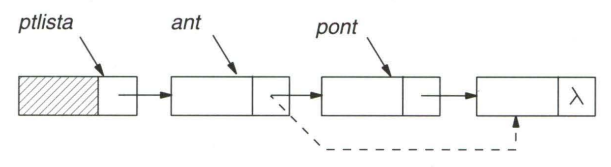
\includegraphics[width=.9\linewidth]{fig/listasimple.png}
\end{center}
\begin{itemize}
\item Percurso unidirecional
\item Remoção necessita de dois ponteiros
\end{itemize}
\end{frame}
\subsection{Dupla}
\label{sec-1-2}
\begin{frame}[label=sec-1-2-1]{\alert{Dois} ponteiros: para os nós anterior e posterior}
\begin{center}
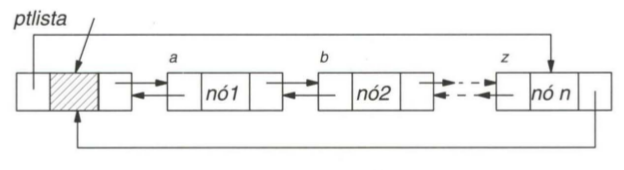
\includegraphics[width=.9\linewidth]{fig/listadoble.png}
\end{center}
\begin{itemize}
\item Percurso bidirecional
\item Remoção necessita de um ponteiro
\end{itemize}
\end{frame}
\subsection{Ordem Crescente}
\label{sec-1-3}
\begin{frame}[label=sec-1-3-1]{Controlado no momento da \alert{inserção}}
\begin{center}
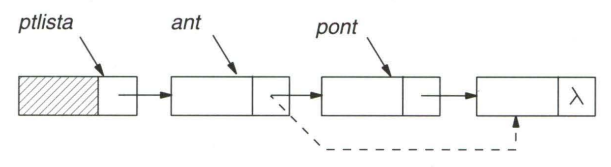
\includegraphics[width=.9\linewidth]{fig/listasimple.png}
\end{center}

\begin{center}
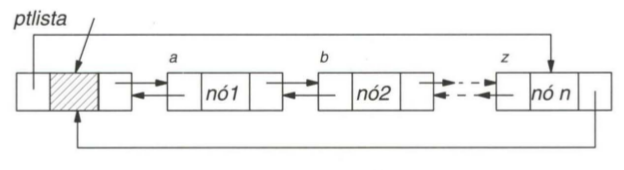
\includegraphics[width=.9\linewidth]{fig/listadoble.png}
\end{center}
\end{frame}
\subsection{Vantagens e Desvantagens}
\label{sec-1-4}
\begin{frame}[label=sec-1-4-1]{Lista Simples}
\begin{center}
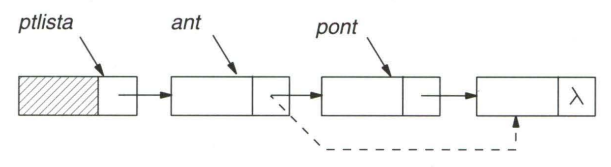
\includegraphics[width=.9\linewidth]{fig/listasimple.png}
\end{center}
\begin{itemize}
\item (+) Menor custo de memória
\item (-) Remoção necessita de dois ponteiros
\item Complexidade do pior caso
\begin{itemize}
\item Percorre a lista completa para inserir/remover (busca)
\item $\mathcal{O}(n)$
\end{itemize}
\end{itemize}
\end{frame}
\begin{frame}[label=sec-1-4-2]{Lista Dupla}
\begin{center}
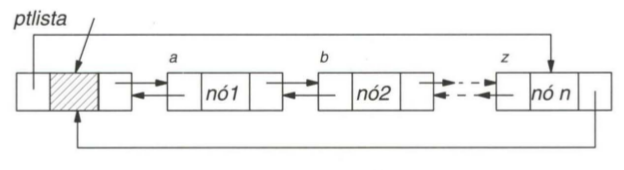
\includegraphics[width=.9\linewidth]{fig/listadoble.png}
\end{center}
\begin{itemize}
\item (+) Inserção imediata na última posição
\item (-) Consome o \alert{dobro} de memória para ponteiros
\item Complexidade do pior caso
\begin{itemize}
\item Percorre a lista até o penúltimo nó para inserir/remover (busca)
\item $\mathcal{O}(n - 1) = \mathcal{O}(n)$
\end{itemize}
\end{itemize}
\end{frame}
\section{Implementação}
\label{sec-2}
\subsection{Descrição do código}
\label{sec-2-1}
\begin{frame}[fragile,label=sec-2-1-1]{Algoritmo}
 \begin{verbatim}
for (qtd = 1; qtd <= MAX; qtd *= 2) { // mais pontos
    for (i = 0; i < (qtd / 2); ++i)   // (1e10)
        l=insercao_enc(rand() % MAX, l);

    time(&inicio_conta);
    for (i = 1; i <= CANT_TESTE; ++i) {
        num = rand() % MAX;
        l=insercao_enc(num,l);
        l=remocion_enc(num,l);
    }
    time(&fim_conta);
    total = fim_conta - inicio_conta;
}
\end{verbatim}
\end{frame}
\begin{frame}[fragile,label=sec-2-1-2]{Algoritmo}
 \begin{verbatim}
for (qtd = 1; qtd <= MAX; qtd *= 2) {    
    for (i = 0; i < (qtd / 2); ++i) // completar a lista
        l=insercao_enc(rand() % MAX, l);

    time(&inicio_conta);
    for (i = 1; i <= CANT_TESTE; ++i) {
        num = rand() % MAX;
        l=insercao_enc(num,l);
        l=remocion_enc(num,l);
    }
    time(&fim_conta);
    total = fim_conta - inicio_conta;
}
\end{verbatim}
\end{frame}
\begin{frame}[fragile,label=sec-2-1-3]{Algoritmo}
 \begin{verbatim}
for (qtd = 1; qtd <= MAX; qtd *= 2) {    
    for (i = 0; i < (qtd / 2); ++i)      
        l=insercao_enc(rand() % MAX, l); // insere números
                                         // aleatórios
    time(&inicio_conta);
    for (i = 1; i <= CANT_TESTE; ++i) {
        num = rand() % MAX;
        l=insercao_enc(num,l);
        l=remocion_enc(num,l);
    }
    time(&fim_conta);
    total = fim_conta - inicio_conta;
}
\end{verbatim}
\end{frame}
\begin{frame}[fragile,label=sec-2-1-4]{Algoritmo}
 \begin{verbatim}
for (qtd = 1; qtd <= MAX; qtd *= 2) {
    for (i = 0; i < (qtd / 2); ++i)      
        l=insercao_enc(rand() % MAX, l); 

    time(&inicio_conta);
    for (i = 1; i <= CANT_TESTE; ++i) { // repetição foi
        num = rand() % MAX;             // necessária
        l=insercao_enc(num,l);          // (1e6)
        l=remocion_enc(num,l);
    }
    time(&fim_conta);
    total = fim_conta - inicio_conta;
}
\end{verbatim}
\end{frame}
\section{Resultados}
\label{sec-3}
\subsection{$t \times n$ --- Lista Simples}
\label{sec-3-1}
\begin{frame}[label=sec-3-1-1]{Lista Simples -- pontos iniciais: rapidez \emph{vs.} precisão}
\begin{center}
\begin{tabular}{rr}
$n$ & $t$\\
\hline
1 & 0\\
2 & 0\\
4 & 0\\
8 & 0\\
16 & 0\\
32 & 0\\
64 & 1\\
128 & 0\\
\end{tabular}
\end{center}
\end{frame}
\begin{frame}[label=sec-3-1-2]{Lista Simples -- a partir de $n = 256$}
\begin{center}
\begin{tabular}{rr}
$n$ & $t$\\
\hline
256 & 2\\
512 & 2\\
1024 & 5\\
2048 & 14\\
4096 & 30\\
8192 & 71\\
16384 & 253\\
32768 & 569\\
65536 & 1338\\
131072 & 5649\\
262144 & 23473\\
524288 & 63852\\
\end{tabular}
\end{center}
\end{frame}
\begin{frame}[label=sec-3-1-3]{Lista Simples -- Gráfico}
\begin{center}
\href{fig/listasimples-log.png}{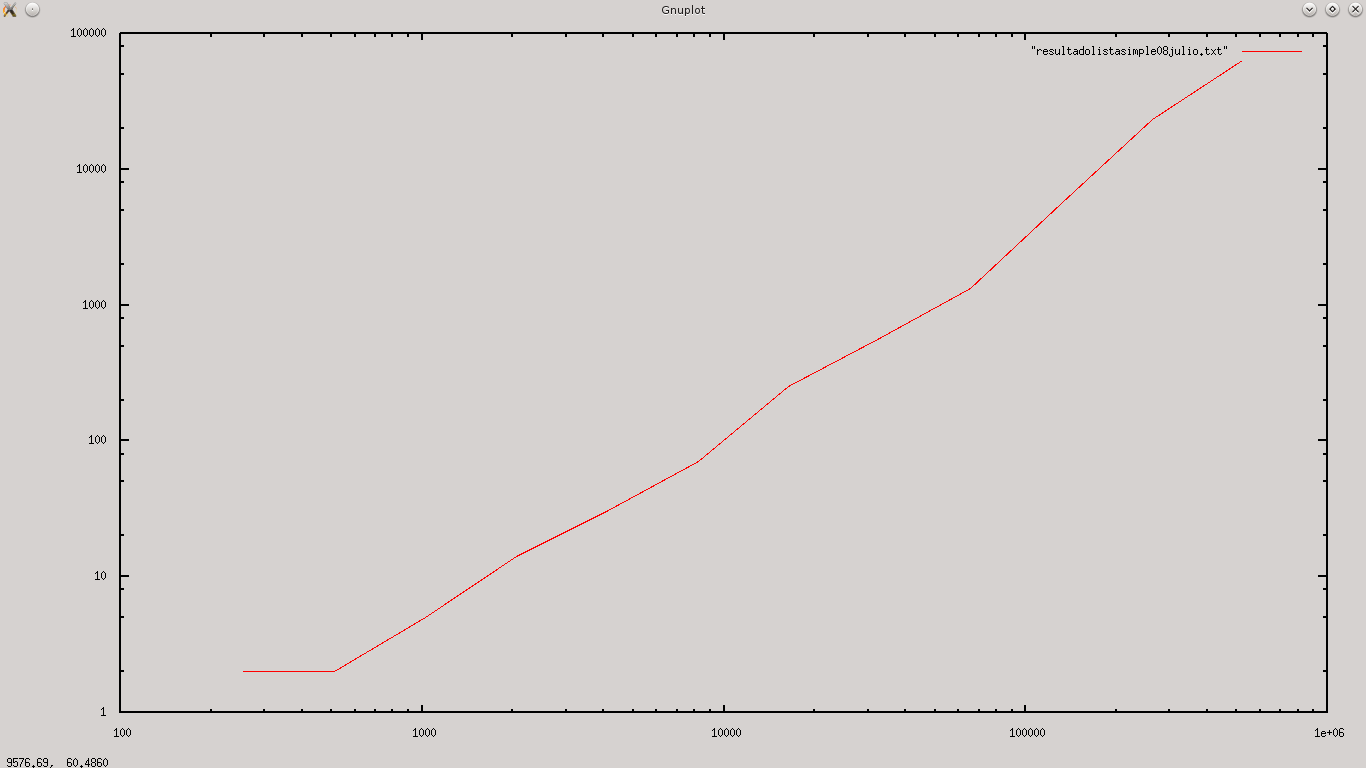
\includegraphics[width=.9\linewidth]{/home/rafaelbeirigo/phd.algo/um/piorcaso/fig/listasimples-log.png}}
\end{center}
\end{frame}
\begin{frame}[label=sec-3-1-4]{Lista Dupla -- pontos iniciais: rapidez \emph{vs.} precisão}
\begin{center}
\begin{tabular}{rr}
$n$ & $t$\\
\hline
1 & 0\\
2 & 0\\
4 & 0\\
8 & 1\\
16 & 0\\
32 & 0\\
64 & 0\\
128 & 1\\
\end{tabular}
\end{center}
\end{frame}
\begin{frame}[label=sec-3-1-5]{Lista Dupla -- a partir de $n = 256$}
\begin{center}
\begin{tabular}{rr}
$n$ & $t$\\
\hline
256 & 2\\
512 & 3\\
1024 & 5\\
2048 & 15\\
4096 & 34\\
8192 & 96\\
16384 & 267\\
32768 & 633\\
65536 & 1560\\
131072 & 6936\\
262144 & 22018\\
524288 & 61744\\
\end{tabular}
\end{center}
\end{frame}
\begin{frame}[label=sec-3-1-6]{Lista Dupla -- Gráfico}
\begin{center}
\href{fig/listasimples-log.png}{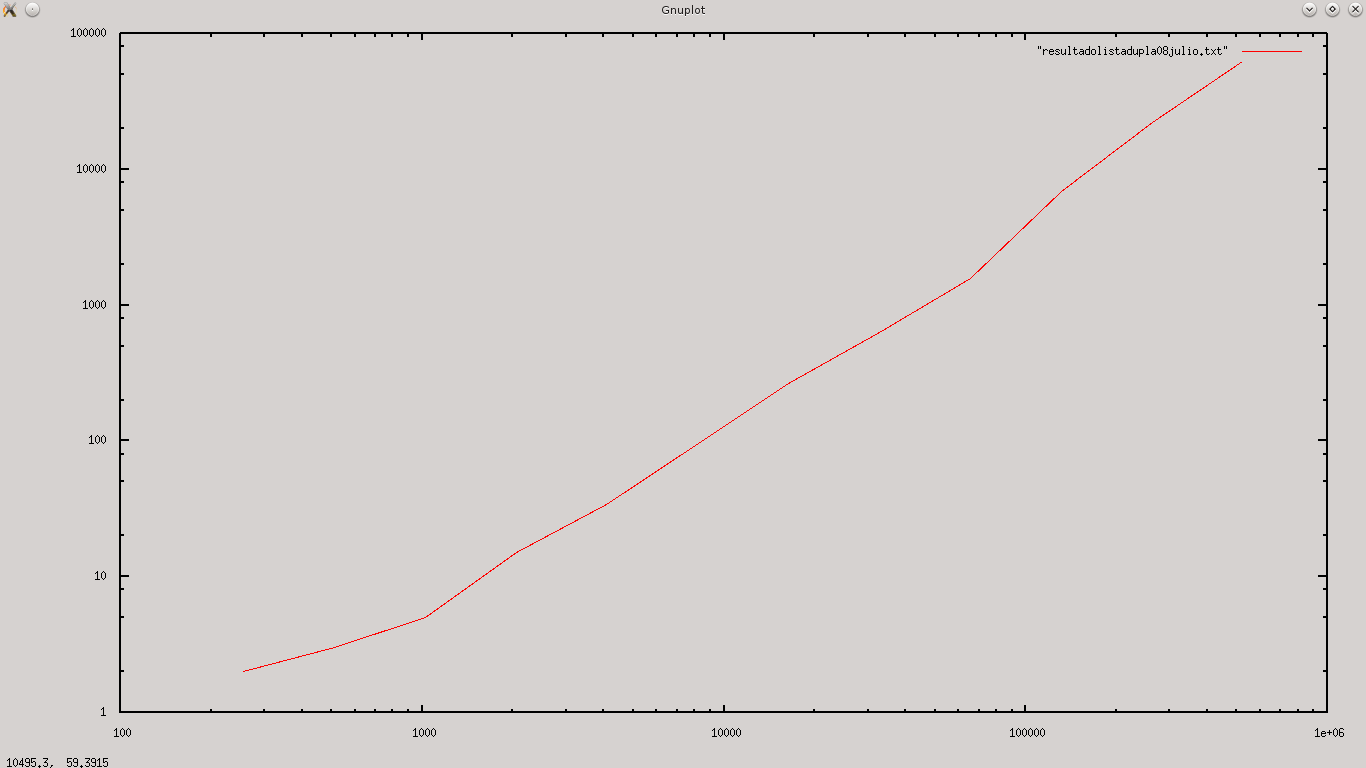
\includegraphics[width=.9\linewidth]{/home/rafaelbeirigo/phd.algo/um/piorcaso/fig/listadupla-log.png}}
\end{center}
\end{frame}
\begin{frame}[label=sec-3-1-7]{Análise: desempenho equiparável (inesperado)}
\begin{center}
\href{fig/compara.png}{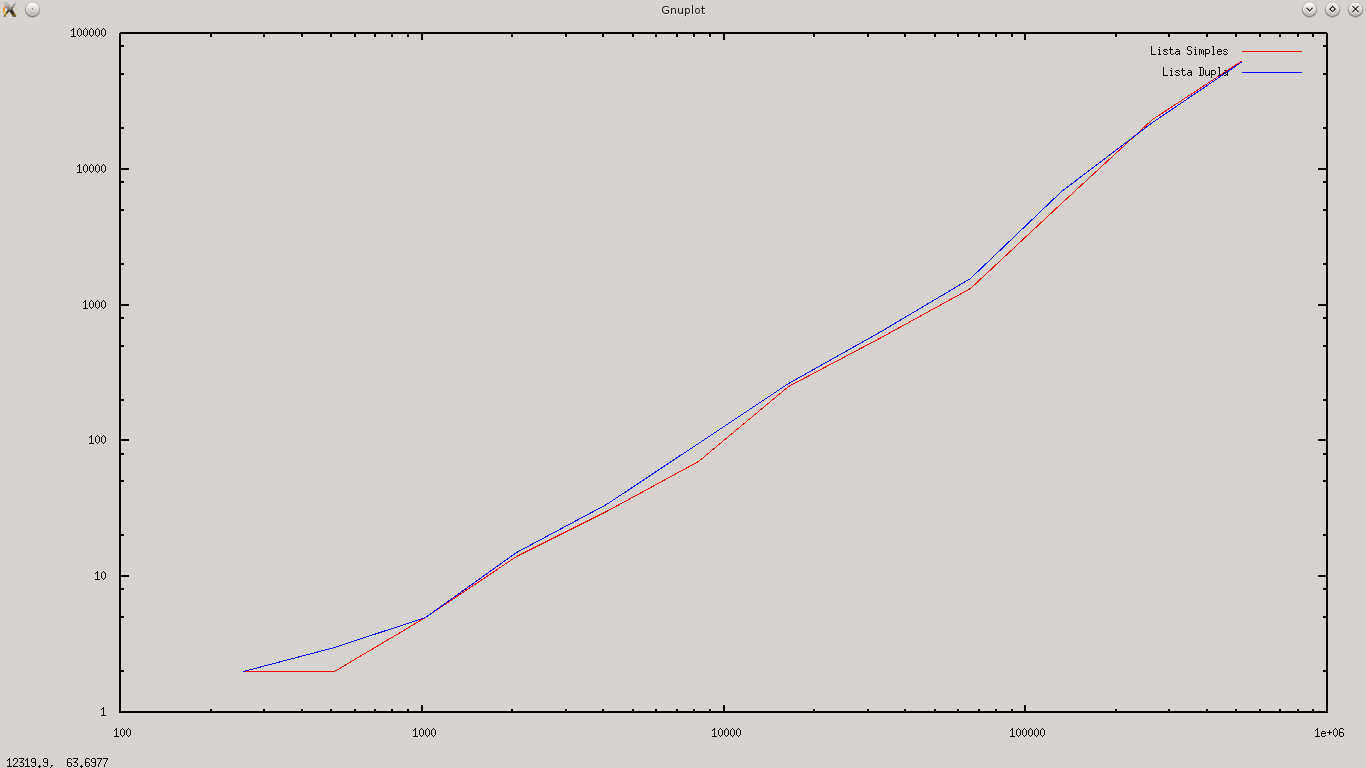
\includegraphics[width=.9\linewidth]{/home/rafaelbeirigo/phd.algo/um/piorcaso/fig/compara.png}}
\end{center}
\end{frame}
\begin{frame}[label=sec-3-1-8]{Possíveis razões}
\begin{itemize}
\item Complexidade teórica considera \alert{pior} caso, i.e., inserção sempre na
última (simples) e penúltima (dupla) posições
\item Experimento realizou inserções de números aleatórios
\begin{itemize}
\item Posições aleatórias
\end{itemize}
\item Resultado corresponde, portanto, à complexidade do \alert{caso médio},
onde se espera que o desempenho seja equiparável
\end{itemize}
\end{frame}
% Emacs 24.5.1 (Org mode 8.2.10)
\end{document}
